\documentclass{beamer}

\usepackage[utf8]{inputenc}
\usepackage[spanish]{babel}
\usepackage{booktabs, makecell, multirow}
\usepackage{graphicx}
\usepackage{tikz}
\usepackage{color, colortbl}
\usepackage[font=tiny,labelfont=bf, format=plain,justification=centering,labelformat=empty]{caption}
\usepackage{fontawesome6}
\usepackage{verbatim}
\usepackage{listings}
\lstset{basicstyle=\ttfamily\footnotesize, language=Bash}
\graphicspath{{./figures}}
\usetheme{CambridgeUS}

\renewcommand\theadfont{\bfseries} % bold tabular headers
\renewcommand\theadalign{ll}
\renewcommand\theadgape{}


\definecolor{mygray}{RGB}{100, 100, 100}
\definecolor{myred}{RGB}{175, 7, 31}
\setbeamercolor{palette primary}{bg=mygray,fg=myred}
\setbeamercolor{palette secondary}{bg=mygray!10!white,fg=myred}
\setbeamercolor{palette tertiary}{bg=myred,fg=white}
\setbeamercolor{block title}{bg=mygray, fg=black}
\setbeamercolor{block title alerted}{bg=myred, fg=white}
\setbeamercolor{block body}{fg=black,bg=mygray!10!white}
\setbeamercolor{block body alerted}{fg=black, bg=myred!10!white}
\setbeamerfont{block body}{size=\small}
\setbeamerfont{block body alerted}{size=\small}
\setbeamerfont{block body example}{size=\small}
\setbeamerfont{block title}{size=\small}
\setbeamerfont{block title alerted}{size=\small}
\setbeamerfont{block title example}{size=\small}
\hypersetup{
  colorlinks,
  allcolors=red,
  urlcolor=blue,
}
\setbeamercolor{section number projected}{bg=mygray,fg=myred}
\setbeamertemplate{itemize item}[triangle]
\setbeamercolor{itemize item}{fg=mygray}
\setbeamertemplate{itemize subitem}[circle]
\setbeamercolor{itemize subitem}{fg=myred!50!white}
\setbeamercolor{section in head/foot}{bg=myred!20!white, fg=mygray}


\title{Curso de Introducción a Git y GitHub}
\subtitle{Día 1 - Introducción}

\author{Héctor Nieto}

\institute{Instituto de Ciencias Agrarias, CSIC}
\date{2026}


\logo{
\includegraphics[height=0.5cm]{CSIC}}

\begin{document}
 \begin{frame}
  \titlepage
 \end{frame}


 \begin{frame}{Programa}
  \small
  \begin{columns}[T]
   \begin{column}{0.33\linewidth}
    \textbf{Día 1: Introducción}
    \begin{itemize}
     \item Importancia del versionado y documentación de software
     \item Qué es Git y la plataforma GitHub
     \item Primeros pasos en Git y GitHub
     \begin{itemize}
      \item Instalación de Git
      \item Configuración de Git, archivos básicos
     \end{itemize}
    \end{itemize}
   \end{column}
   \begin{column}{0.33\linewidth}
    \textbf{Día 2: Iniciación a Git}
    \begin{itemize}
     \item Crear repositorios
     \item Control de cambios y versionado
     \item Restaurar versiones previas (\texttt{checkout} y \texttt{restore})
     \item Ramificaciones (\texttt{branch}) del código
     \item Actualizar el repositorio  local y remoto
    \end{itemize}
   \end{column}
   \begin{column}{0.33\linewidth}
    \textbf{Día 3: Git colaborativo}
    \begin{itemize}
     \item Fusionado y resolución de conflictos
     \begin{itemize}
      \item Fusionado de ramificaciones
      \item Resolución de conflictos
     \end{itemize}
     \item Código colaborativo en GitHub
     \begin{itemize}
      \item Creación de copias (\texttt{forks})
      \item Sugerencias de cambios (\texttt{Pull requests})
     \end{itemize}
    \end{itemize}
   \end{column}
  \end{columns}
 \end{frame}


 \begin{frame}{¿Qué es Git?}
  GIT - the stupid content tracker (Linus Torvalds)

  ``git'' can mean anything, depending on your mood.
  \begin{itemize}
   \item random three-letter combination that is pronounceable, and not actually used by any common UNIX command.  The fact that it is a mispronounciation of "get" may or may not be relevant.
   \item stupid. contemptible and despicable. simple. Take your pick from the dictionary of slang.
   \item “Global Information Tracker": you're in a good mood, and it actually works for you. Angels sing, and a light suddenly fills the room.
   \item "Goddamn Idiotic Truckload of sh*t": when it breaks
  \end{itemize}

		\url{https://github.com/git/git/blob/master/README.md}
 \end{frame}


 \begin{frame}{¿Qué es Git?}
  \begin{columns}[T]
   \begin{column}{0.66\textwidth}
    \texttt{Git} is British slang for ``pig headed, think they are always correct, argumentative''.
				\vspace{1cm}
    Linus Torvalds: ``I'm an egotistical bastard, and I name all my projects after myself. First \texttt{Linux}, now \texttt{Git}''

    \vspace{1cm}
    \url{https://tinyurl.com/4vduybkm}
   \end{column}
   \begin{column}{0.33\textwidth}\centering
    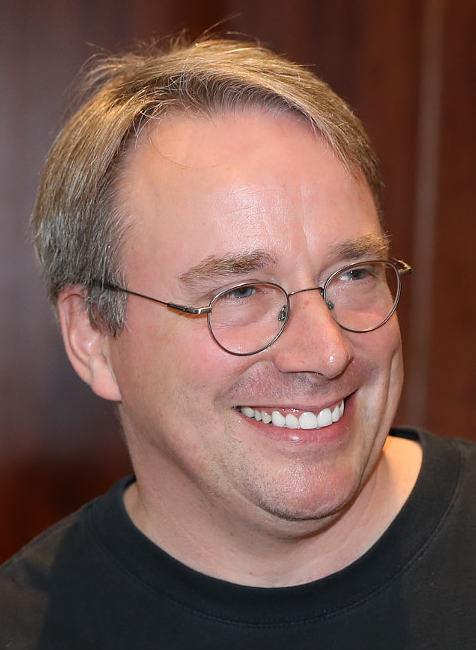
\includegraphics[width=\columnwidth]{01_linus_torvalds}
   \end{column}
  \end{columns}
 \end{frame}

 \begin{frame}{¿Por qué Git?}
  \begin{columns}[T]
   \begin{column}{0.5\textwidth}
    Sistema de versionado y control de contenidos
    \begin{itemize}
     \item Código
     \item Datos
     \item Texto
    \end{itemize}
   \end{column}
   \begin{column}{0.5\textwidth}
    Sistema de versionado y control de contenidos
    \begin{itemize}
     \item Rápido
     \item Diseño sencillo
		   \item Desarrollo no lineal -  en ramas paralelas
		   \item Totalmente distribuido
		   \item Capaz de manejar grandes proyectos eficientemente (núcleo \texttt{kernel} de Linux)
    \end{itemize}
   \end{column}
  \end{columns}
  \begin{alertblock}<2->{Fundamental Documentar Código y sus Cambios}
  \end{alertblock}
 \end{frame}


 \begin{frame}{¿Cómo funciona Git?}
  Versionado
  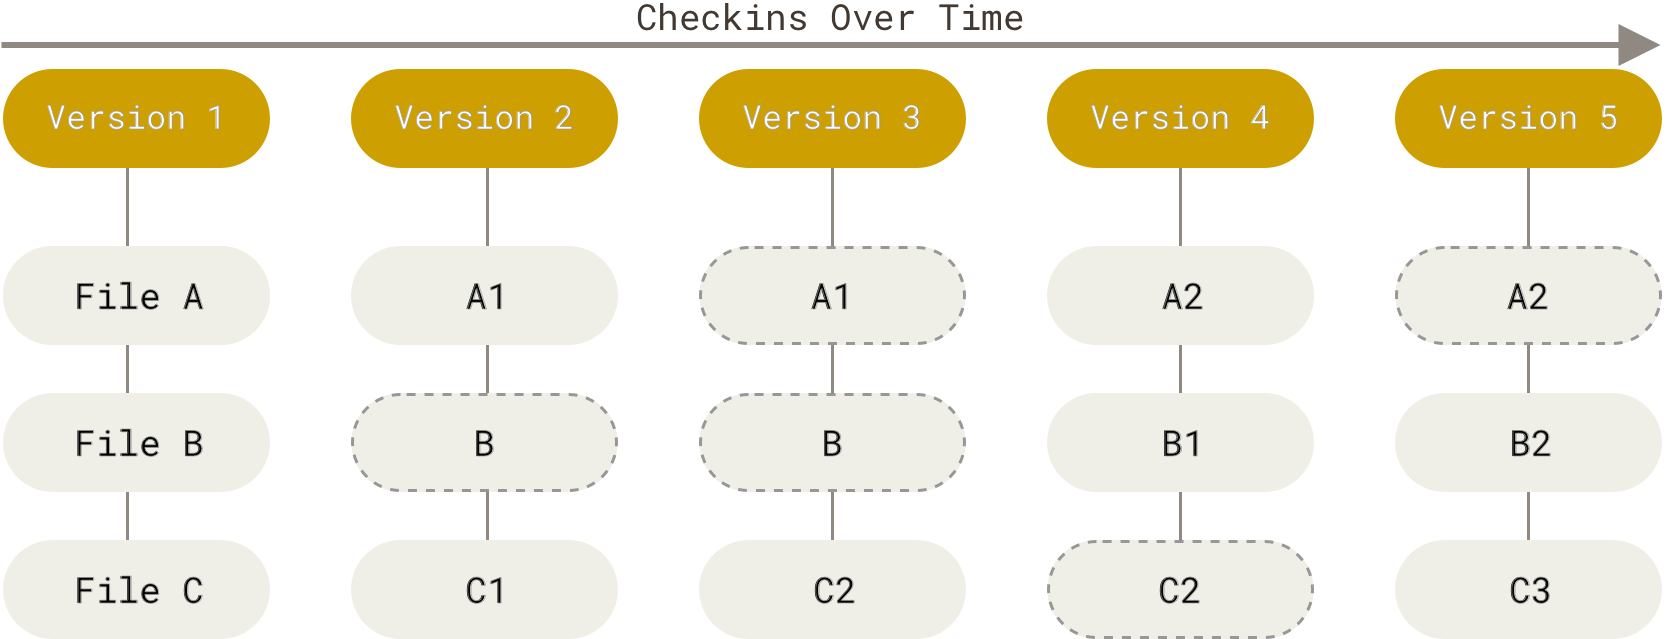
\includegraphics[width=\textwidth]{01_versioning}
  Chacon \& Straub (2021) Pro Git
 \end{frame}


 \begin{frame}{¿Cómo funciona Git?}
  \begin{columns}
   \begin{column}{0.5\textwidth}
    Distribución descentralizada
    \begin{itemize}
     \item Cada repositorio local es una réplica / copia de seguridad
     \item Si el servidor falla cualquier otra copia local puede usarse como reemplazo
    \end{itemize}
    \vspace{2cm}
    Chacon \& Straub (2021) Pro Git
   \end{column}
   \begin{column}{0.5\textwidth}\centering
    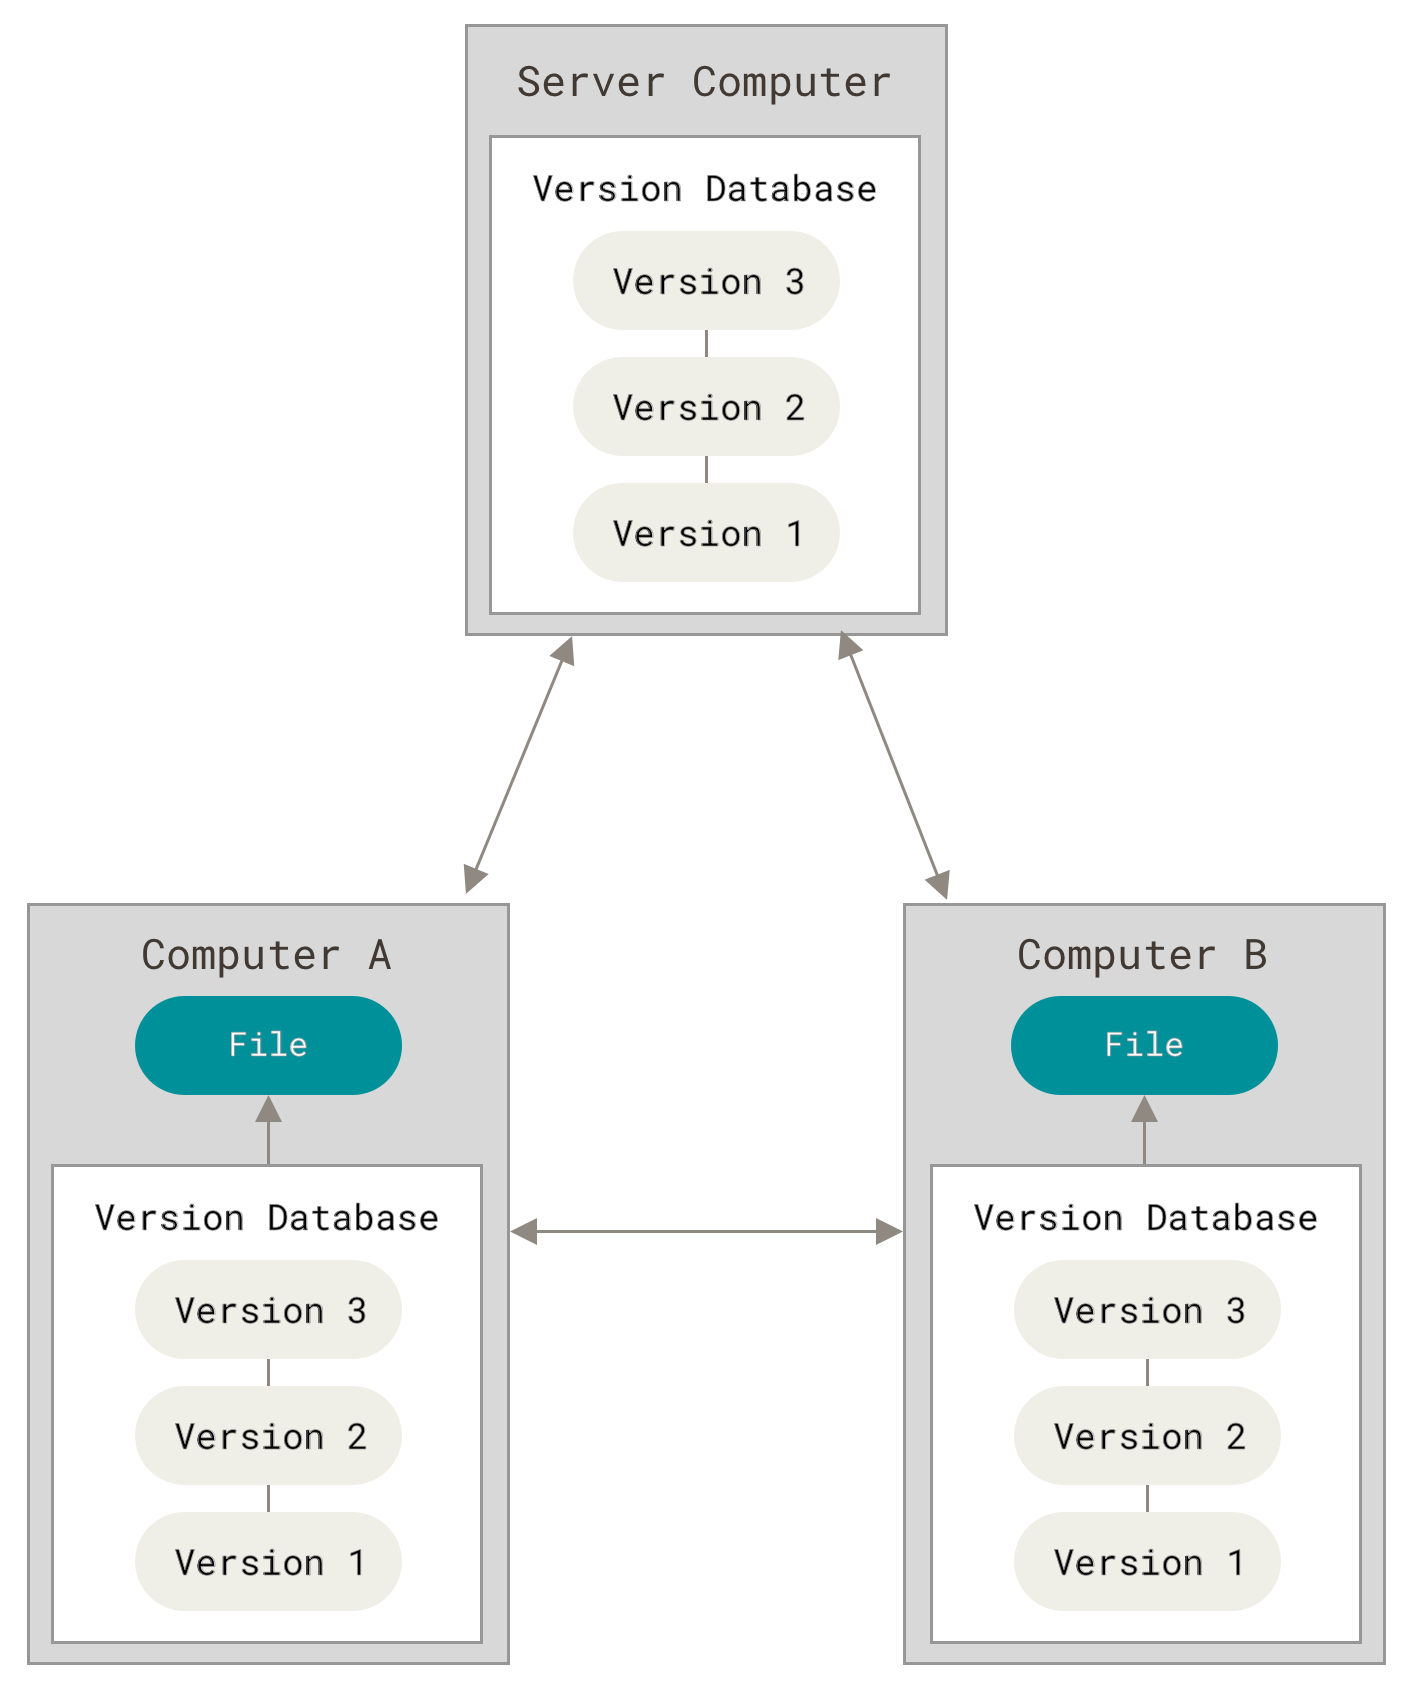
\includegraphics[width=\columnwidth]{01_distributed_version_control}
   \end{column}
  \end{columns}
 \end{frame}


 \begin{frame}{¿Qué es GitHub?}
  \begin{columns}[T]
   \begin{column}{0.5\textwidth}
    Plataforma online de repositorios Git
    \begin{itemize}
     \item Hace la función de servidor remoto del código
    \end{itemize}
    Propiedad de Microsoft
    \begin{itemize}
     \item Con ánimo de lucro
    \end{itemize}
    Ayuda:
    \begin{itemize}
     \item Trabajo colaborativo
     \item Diseminación de código abierto
     \item Herramientas para la difusión y transferencia
    \end{itemize}
   \end{column}
   \begin{column}{0.5\textwidth}\centering
    \begin{tikzpicture}
     \node[inner sep=0] (big) at (0,0)
        {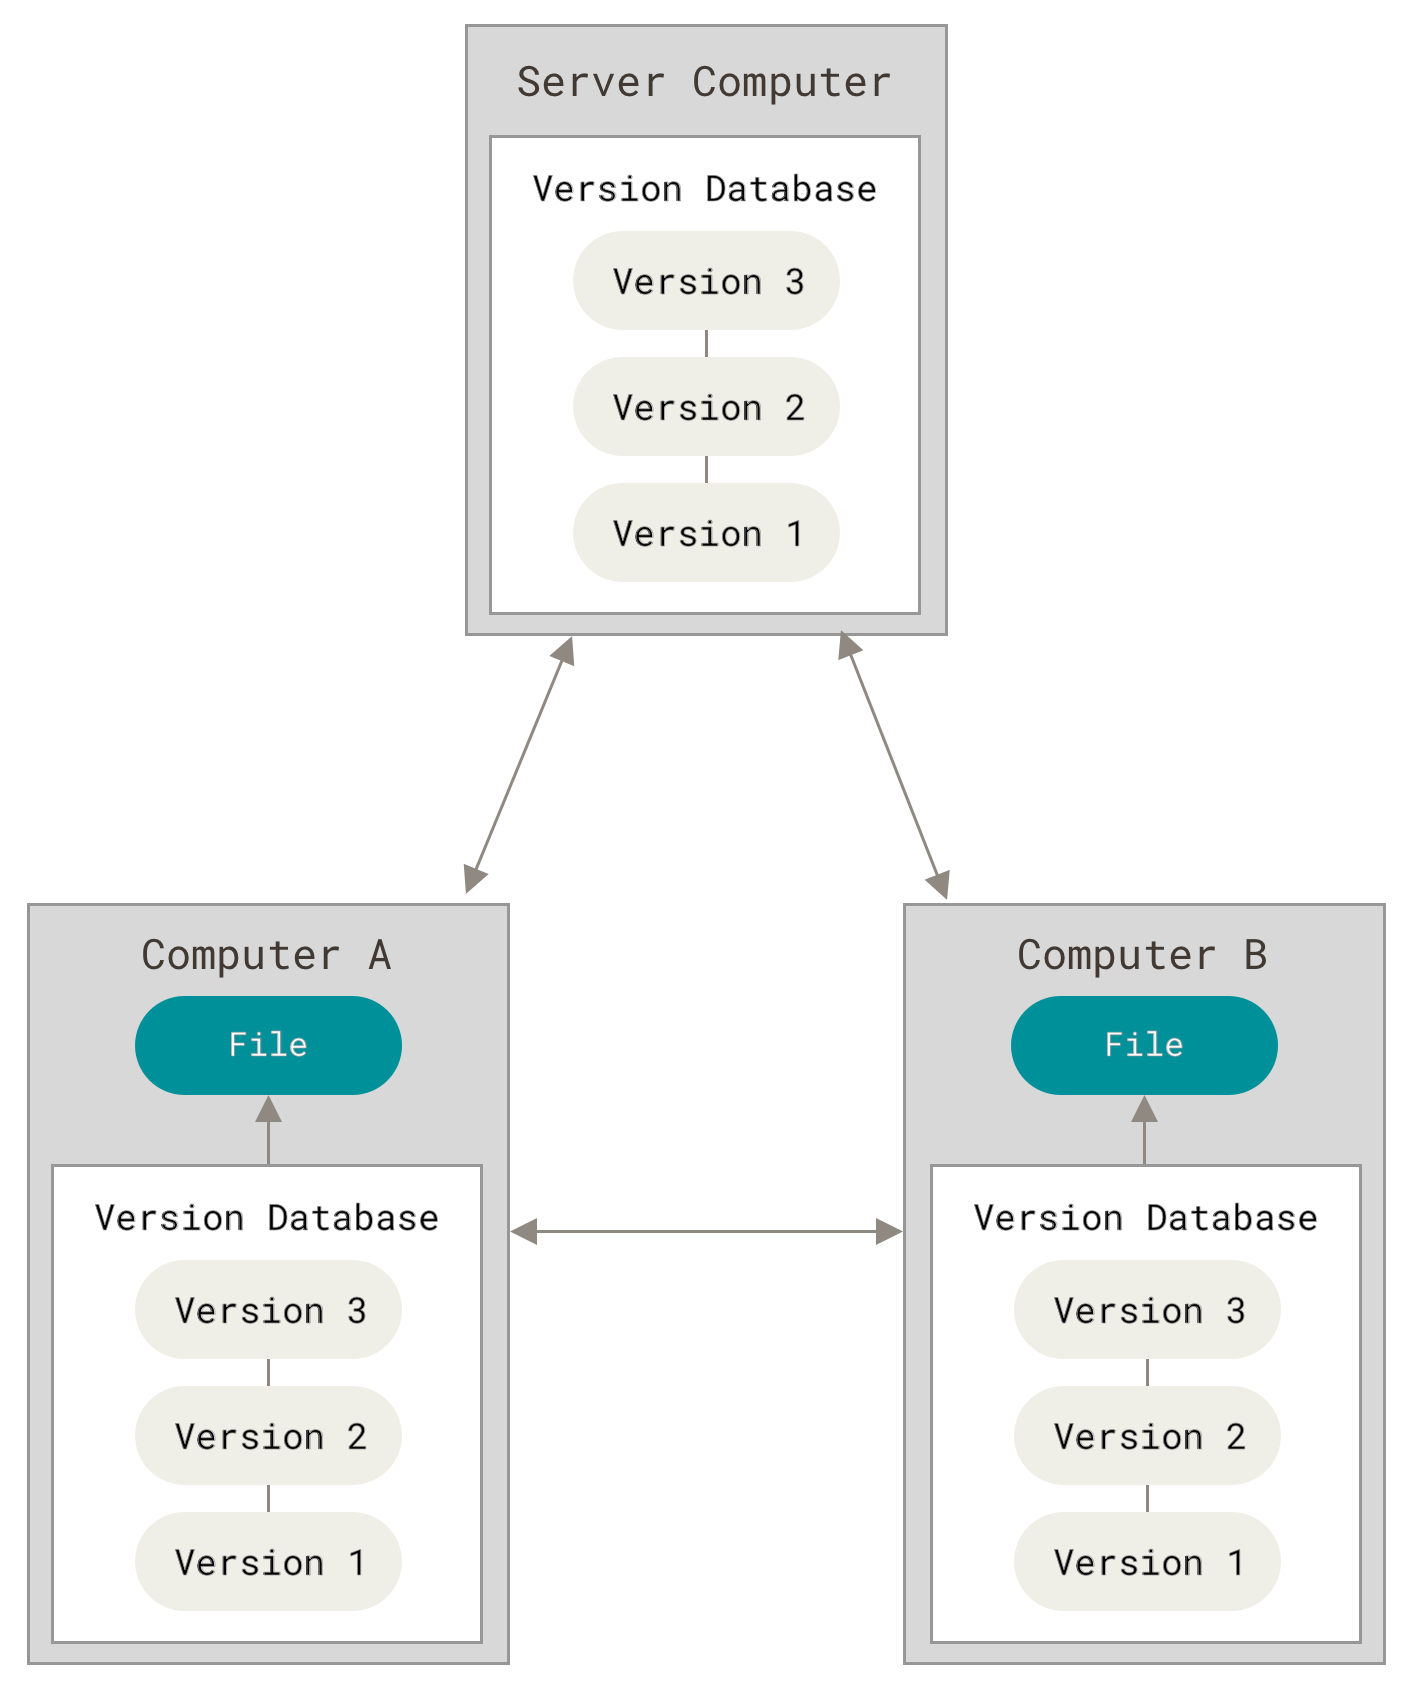
\includegraphics[width=\columnwidth]{01_distributed_version_control}};
     \node[minimum width=\columnwidth, anchor=south, fill=white] (small) at ([yshift=0cm]big.south)
        {
\includegraphics[height=0.4\textheight]{01_github}};
    \end{tikzpicture}
   \end{column}
  \end{columns}
 \end{frame}


 \begin{frame}{Git y GitHub}
	 \begin{columns}
	  \begin{column}{0.6\textwidth}
	   \begin{block}{Nota}
	    Puedes usar sin problema \texttt{Git} sin necesidad de \texttt{GitHub}
	   \end{block}
	   \begin{alertblock}{Importante}
	    Si usas \texttt{GitHub} tienes que conocer \texttt{Git}
	   \end{alertblock}
	   \begin{block}{Alternativas a GitHub}
	    \begin{itemize}
		    \item \href{https://gitlab.com}{GitLab}
		    \item \href{https://bitbucket.org/}{Bitbucket}
		    \item servidor propio
		   \end{itemize}
	   \end{block}
	  \end{column}
	  \begin{column}{0.4\textwidth}
	   
\includegraphics[width=\columnwidth]{01_gitlab}
	  \end{column}
	 \end{columns}
 \end{frame}


	\begin{frame}{Add-ons de GitHub}
	 \begin{columns}[T]
	  \begin{column}{0.6\textwidth}
	   Generación de DOIs
	   \begin{itemize}
	    \item \url{https://zenodo.org/}
	    \item \url{https://guides.github.com/activities/citable-code/}
	   \end{itemize}
	   Documentación de software online
	   \begin{itemize}
	    \item \url{https://readthedocs.org/}
	    \item \url{https://github.com/readthedocs/readthedocs.org}
	   \end{itemize}
    Servicio de páginas web
    \begin{itemize}
     \item \url{https://docs.github.com/en/pages}
    \end{itemize}
	  \end{column}
	  \begin{column}{0.4\textwidth}\centering
	   
\includegraphics[width=\columnwidth, height=0.2\textheight, keepaspectratio]{01_zenodo}\\
	   \vspace{0.5cm}
	   
\includegraphics[width=\columnwidth, height=0.2\textheight, keepaspectratio]{01_readthedocs}\\
	   
\includegraphics[width=\columnwidth, height=0.4\textheight, keepaspectratio]{01_github-pages}
	  \end{column}
	 \end{columns}
	\end{frame}


		\begin{frame}{Mis ``Mandamientos'' de Git}
	 \begin{columns}[T]
	  \begin{column}{0.7\textwidth}
	   Adaptado de \href{https://peps.python.org/pep-0020/}{PEP 20 -- The Zen of Python}
	   \begin{itemize}
	    \item Beautiful is better than ugly.
	    \item Explicit is better than implicit.
	    \item Simple is better than complex.
	    \item Simple is better than complicated.
	    \item Flat is better than nested.
	    \item Readability counts.
	    \item Special cases aren't special enough to break the rules.
	    \item Errors should never pass silently.
	    \item Now is better than never.
	    \item Although never is often better than \alert{right} now.
	   \end{itemize}
	  \end{column}
	  \begin{column}{0.3\textwidth}\centering
	   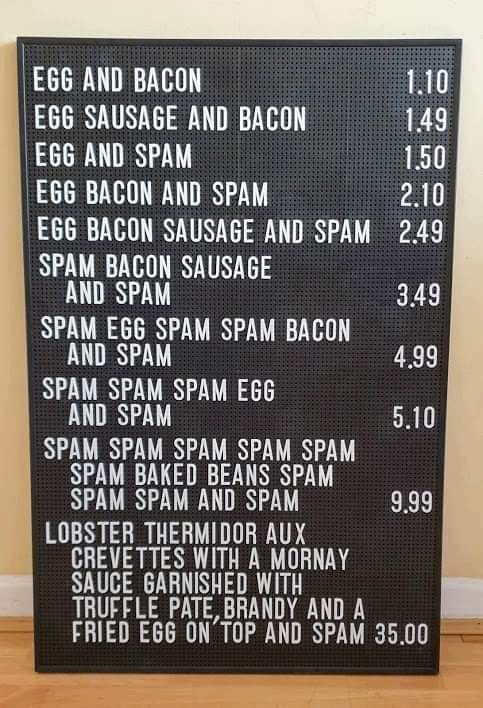
\includegraphics[width=\columnwidth, keepaspectratio]{01_spam}
	   \url{https://vimeo.com/329001211}
	  \end{column}
	 \end{columns}
	\end{frame}

	\begin{frame}{Documentación y legibilidad}
	 ``Code is more often read than written'' (Guido van Rossum)
	 \begin{columns}[T]
	  \begin{column}{0.6\textwidth}
	   \alert{Máximo 79 caracteres por línea}
	   Python
	   \begin{itemize}
	    \item Guía de estilo para Python: \url{https://peps.python.org/pep-0008/}
	    \item Guía de estilo de Numpy docstrings: \url{https://numpydoc.readthedocs.io/en/latest/format.html}
	   \end{itemize}
   \end{column}
   \begin{column}{0.4\textwidth}
    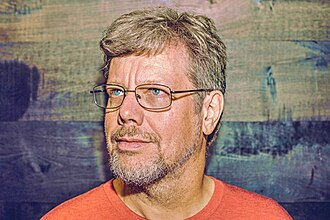
\includegraphics[width=\columnwidth]{01_guido_van_rossum}
   \end{column}
	 \end{columns}
		 R
		 \begin{itemize}
		  \item Roxygen2 docstrings: \url{https://github.com/r-lib/roxygen2}
		 \end{itemize}
		 C
		 \begin{itemize}
		  \item Guía de estilos para C: \url{https://peps.python.org/pep-0007/}
		 \end{itemize}
	\end{frame}

\end{document}
